%\usepackage[graphicx]
\documentclass{beamer}
\usetheme{Warsaw}
\begin{document}

\begin{frame}{AND GATE}
\begin{block}{}
    \begin{itemize}
	\item A logic gate is a physical device that implements a Boolean function
	\item It performs a logical operation on one or more logic inputs and produces a single logic output.
	\item AND gate takes two inputs and gives output as low(0) whenever any of its input is low(0).   
	\item The representation of \alert{AND} function is \alert{C=A.B} 
    \end{itemize}
  \end{block}
\pause
\begin{block}{Truth Table for AND gate}
\begin{tabular}{|c|c||c|}
\hline
 \textbf{A} &
\textbf{B} & \textbf{C} \\
\hline
\hline
 0 & 0 & 0 \\
\hline
 0 & 1 & 0 \\
\hline
 1 & 0 & 0 \\
\hline
 1 & 1 & 1 \\
\hline
\end{tabular}
\end{block}
\end{frame}
\begin{frame}
\begin{figure}
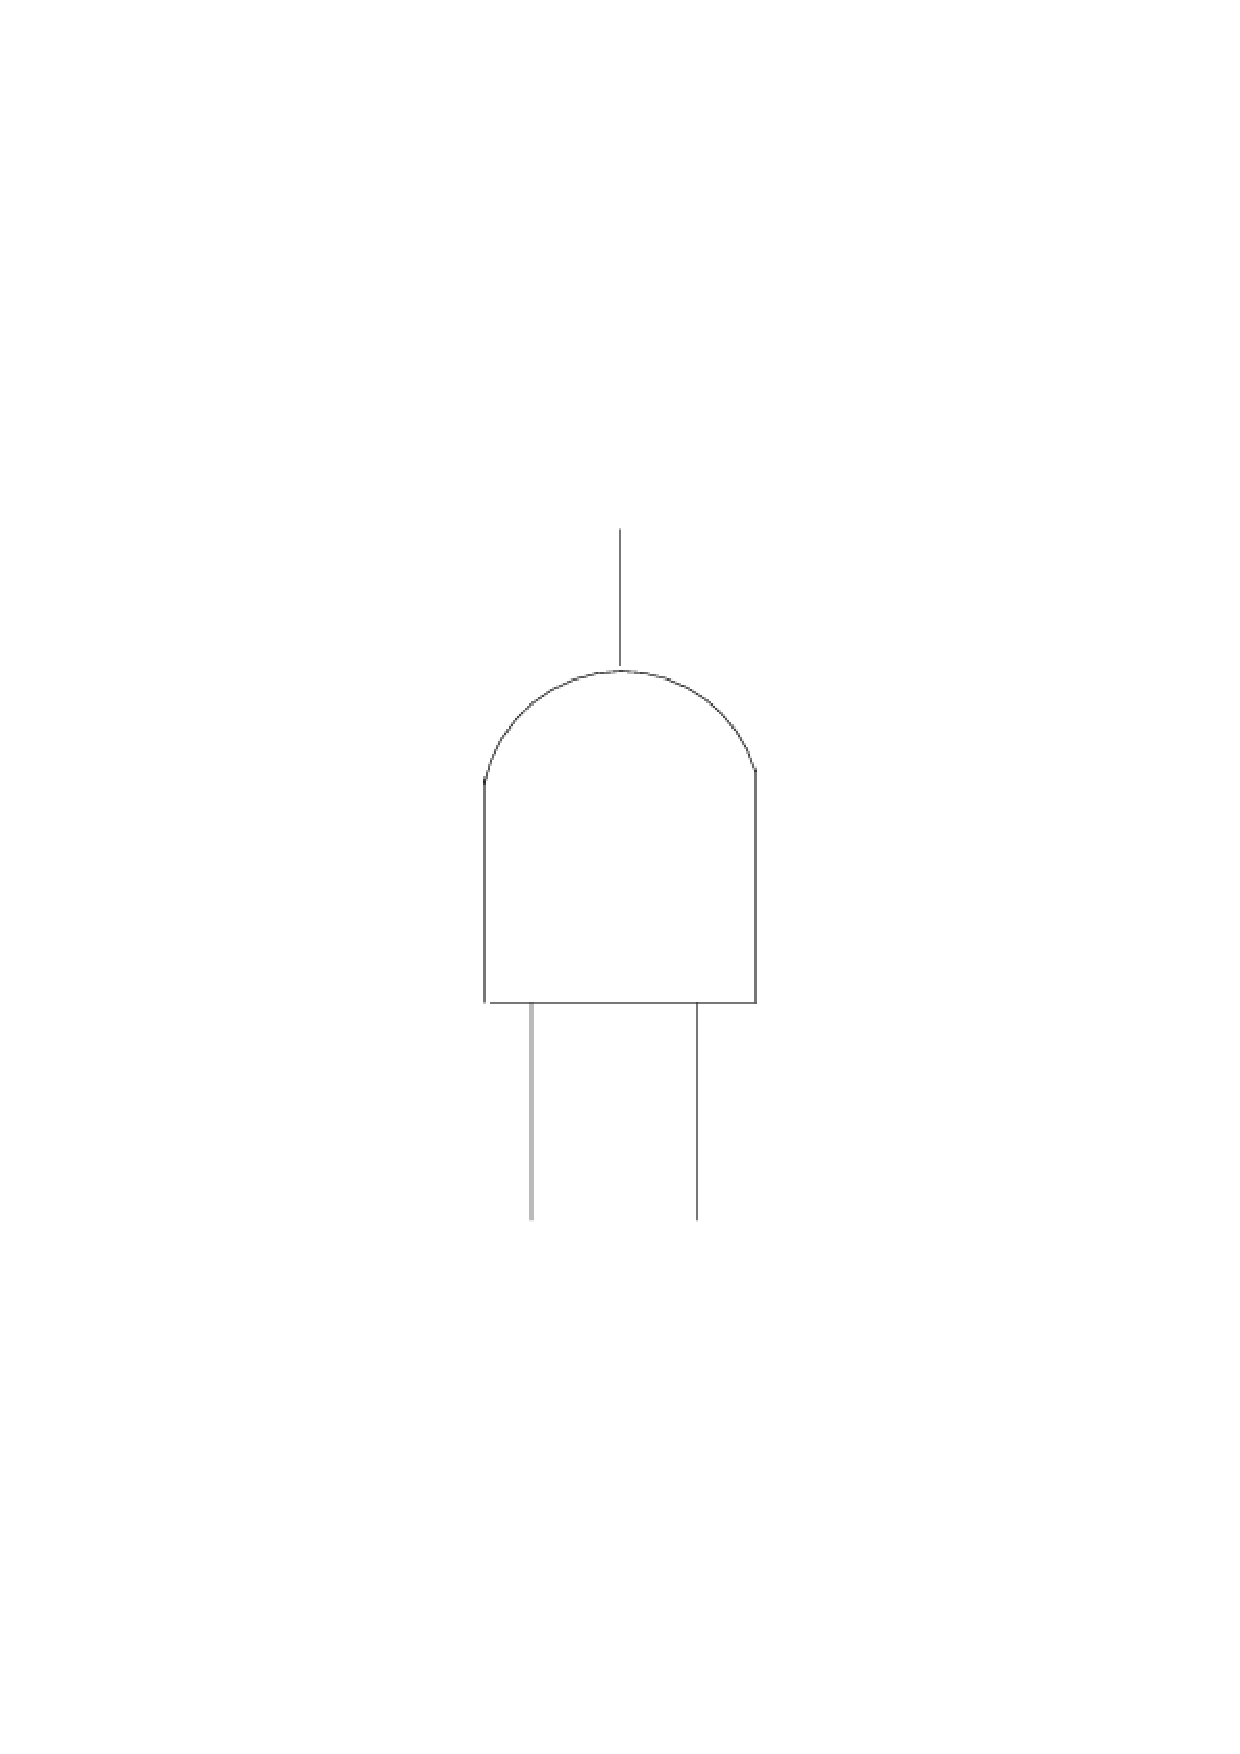
\includegraphics[scale=0.4]{../Desktop/251/event/beamer_bib/and} 
\end{figure}
\end{frame}
\begin{frame}{OR GATE}
\begin{block}{}
\begin{itemize}
  \item OR gate takes two inputs and gives output as high(1) whenever any of it's input is high(1),else it gives low(0).
  \item It is represented as \alert{C=A+B}
\end{itemize}
\end{block}
\medskip
\medskip
\pause
\begin{block}{Truth Table for OR gate}
\begin{tabular}{|c|c||c|}
\hline
 \textbf{A} &
\textbf{B} & \textbf{C} \\
\hline
\hline
 0 & 0 & 0 \\
\hline
 0 & 1 & 1 \\
\hline
 1 & 0 & 1 \\
\hline
 1 & 1 & 1 \\
\hline
\end{tabular}
\end{block}
\end{frame}
\begin{frame}{NOT GATE}
\begin{block}{}
\begin{itemize}
  \item NOT gate is different from previous two in the sense that it has 1 input instead of two.
  \item The output is high(1) if input is low(0) and vice versa.
\end{itemize}
\end{block}
\medskip
\medskip
\pause
\begin{block}{Truth Table for NOT gate}
\begin{tabular}{|c|c|}
\hline
 \textbf{A} &
\textbf{B} \\
\hline
\hline
 0 & 1 \\
\hline
 1 & 0 \\
\hline
\end{tabular}
\end{block}
\end{frame}
\begin{frame}{De-Morgan's Laws}
The rules given by De-Morgan allow the expression of conjunctions and disjunctions purely in terms of each other via negation.
\pause
\begin{block}{Laws}
The laws if laid in plain English are as follows:
\begin{enumerate}
\item The negation of a conjunction is the disjunction of the negations.
\item The negation of a disjunction is the conjunction of the negations.
\end{enumerate}
\end{block}
\end{frame}
\begin{frame}{Law 1}
\begin{theorem}
The negation of a conjunction is the disjunction of the negations.\\
Represented mathematically:
\begin{equation}
\overline{A+B}=\overline{A}.\overline{B}
\end{equation}
\end{theorem}
\end{frame}
\begin{frame}{Law 2}
\begin{theorem}
The negation of a disjunction is the conjunction of the negations.\\
Represented mathematically:
\begin{equation}
\overline{A.B}=\overline{A}+\overline{B}
\end{equation}
\end{theorem}
\end{frame}
\end{document}

